\documentclass[a4paper,11pt]{article}
\usepackage{amsmath}
\usepackage[english]{babel}
\usepackage{color}
\usepackage{graphicx}
\usepackage{hyperref}
\usepackage{mathabx}

\DeclareMathOperator*{\argmax}{arg\,max}
\DeclareMathOperator*{\Bern}{Bern}
\newcommand{\V}[1]{\ensuremath{\mathbf{#1}}}
\newcommand{\T}[1]{\ensuremath{\mathtt{#1}}}
\newcommand{\mean}{\ensuremath{\boldsymbol{\mu}}}
\newcommand{\cov}{\ensuremath{\boldsymbol{\Sigma}}}
\newcommand{\npdf}{\ensuremath{\mathcal{N}}}

\newcommand{\hl}[1]{\colorbox{cyan}{#1}}
\newcommand{\mhl}[1]{\mathchoice%
  {\colorbox{cyan}{$\displaystyle#1$}}%
  {\colorbox{cyan}{$\textstyle#1$}}%
  {\colorbox{cyan}{$\scriptstyle#1$}}%
  {\colorbox{cyan}{$\scriptscriptstyle#1$}}}

\title{Lab 4: Gaussian Processes}
\author{Patrick de Kok}
\begin{document}
\maketitle

In this exercise, I have learnt how to use Gaussian processes on sparse data, such as the \texttt{chirps.mat} dataset.  The data has been split in a train set of 12 data points and a test set of 3 data points.  The data points have been randomly divided into either set.


\section{The Gaussian distribution}
\begin{figure}
  \begin{center}
    \caption[Plot of the Gaussian distribution with covariance $\cov_{1,1} = 1, \cov_{2,2} = 3$.]{Plot of the Gaussian distribution with mean $\mean = 0$ and covariance $\cov = \begin{bmatrix}1 & 0\\0 & 3\end{bmatrix}$.  In the plot above, one can see the contour plot of $\mathcal G_1 = \npdf(\V{x} ; \mean, \cov)$ with isolines for points with probability density $0.01, 0.02, \ldots 0.09$.  The lower plot shows the marginal distribution over $x_1$.}
    \label{fig:plot1}
    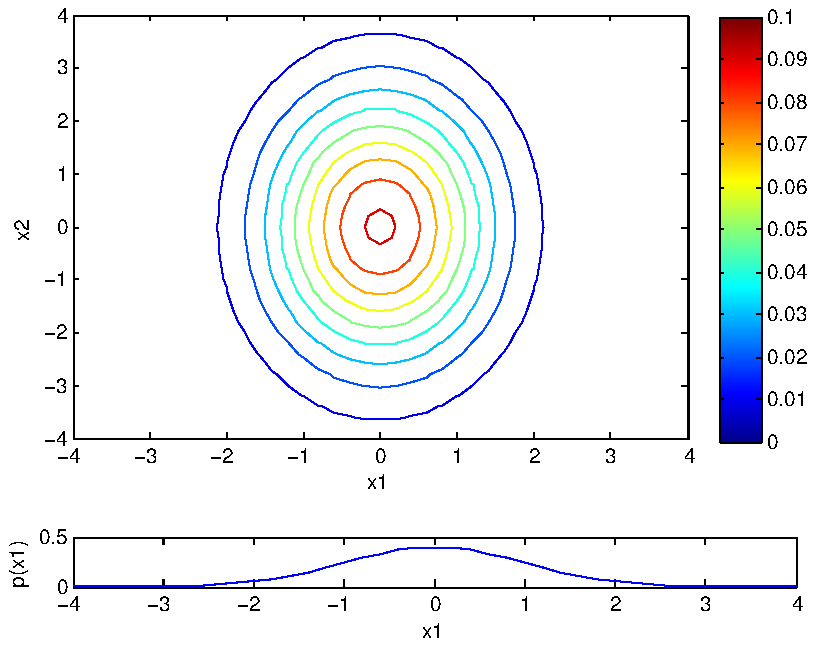
\includegraphics[width=0.8\textwidth]{ex1plot1}
  \end{center}
\end{figure}
\begin{figure}
  \begin{center}
    \caption{Plots of the conditional distribution over $x_1$ given various values for $x_2$ given the Gaussian distribution $\mathcal G_1$.  The conditional distribution over $x_1$ is plotted from top to bottom for $x_2 = -3$, $x_2 = -2$, $x_2 = -1$, $x_2 = 0$, $x_2 = 1$, $x_2 = 2$ and $x_2 = 3$.}
    \label{fig:plot2}
    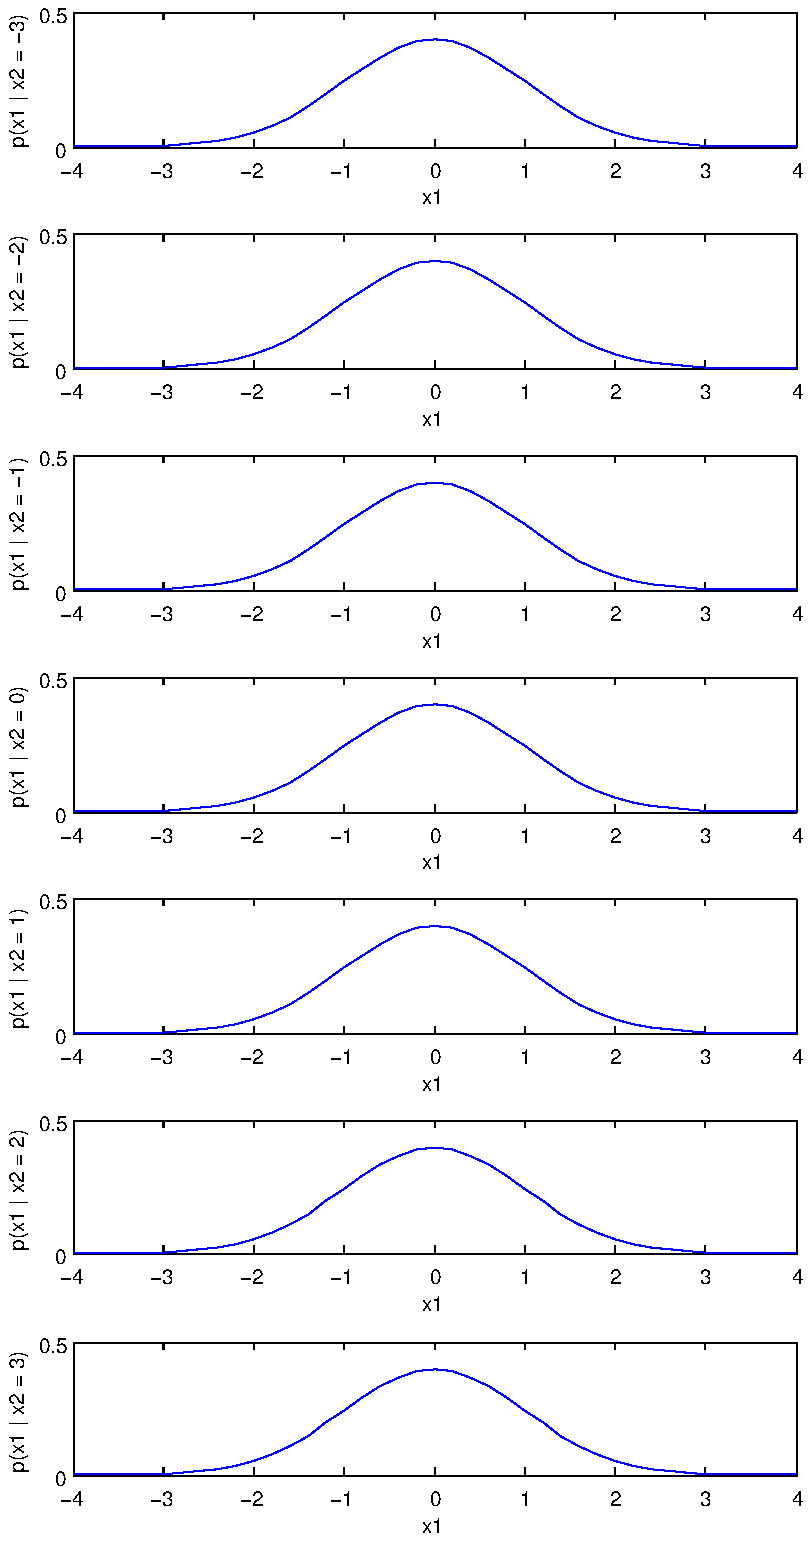
\includegraphics[width=0.8\textwidth]{ex1plot2}
  \end{center}
\end{figure}
\begin{figure}
  \begin{center}
    \caption[Surface plot of the Gaussian distribution with covariance $\cov_{1,1} = \cov_{2,2} = 1, \cov_{1,2} = \cov_{2,1} = 0.7$.]{Surface plot of the Gaussian distribution $\mathcal G_2 = \npdf(\V{x}; \mean, \cov)$ with mean $\mean = 0$ and covariance $\cov = \begin{bmatrix}1 & 0.7\\0.7 & 1\end{bmatrix}$.}
    \label{fig:plot3}
    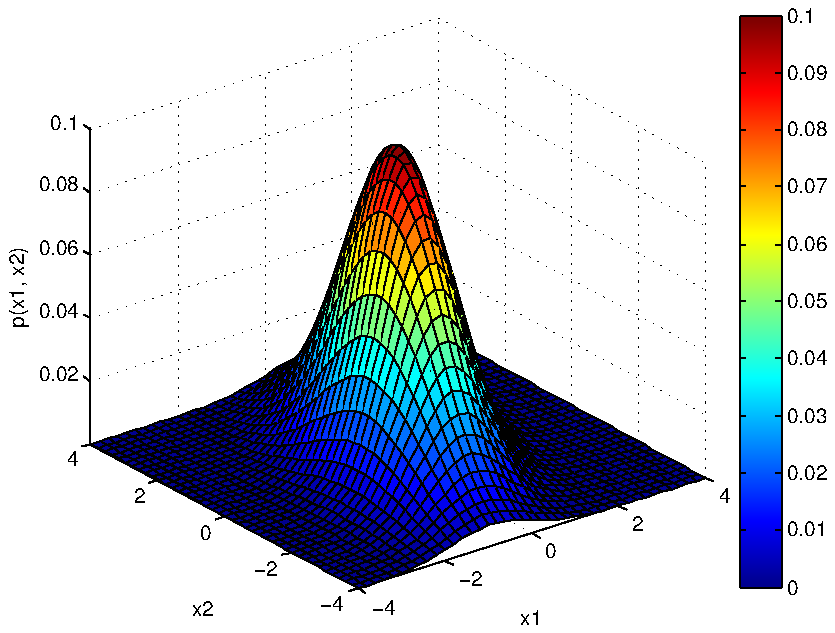
\includegraphics[width=0.8\textwidth]{ex1plot3}
  \end{center}
\end{figure}
\begin{figure}
  \begin{center}
    \caption{Plots of the conditional distribution over $x_1$ given various values for $x_2$ given the Gaussian distribution $\mathcal G_2$.  The conditional distribution over $x_1$ is plotted from top to bottom for $x_2 = -3$, $x_2 = -2$, $x_2 = -1$, $x_2 = 0$, $x_2 = 1$, $x_2 = 2$ and $x_2 = 3$.}
    \label{fig:plot4}
    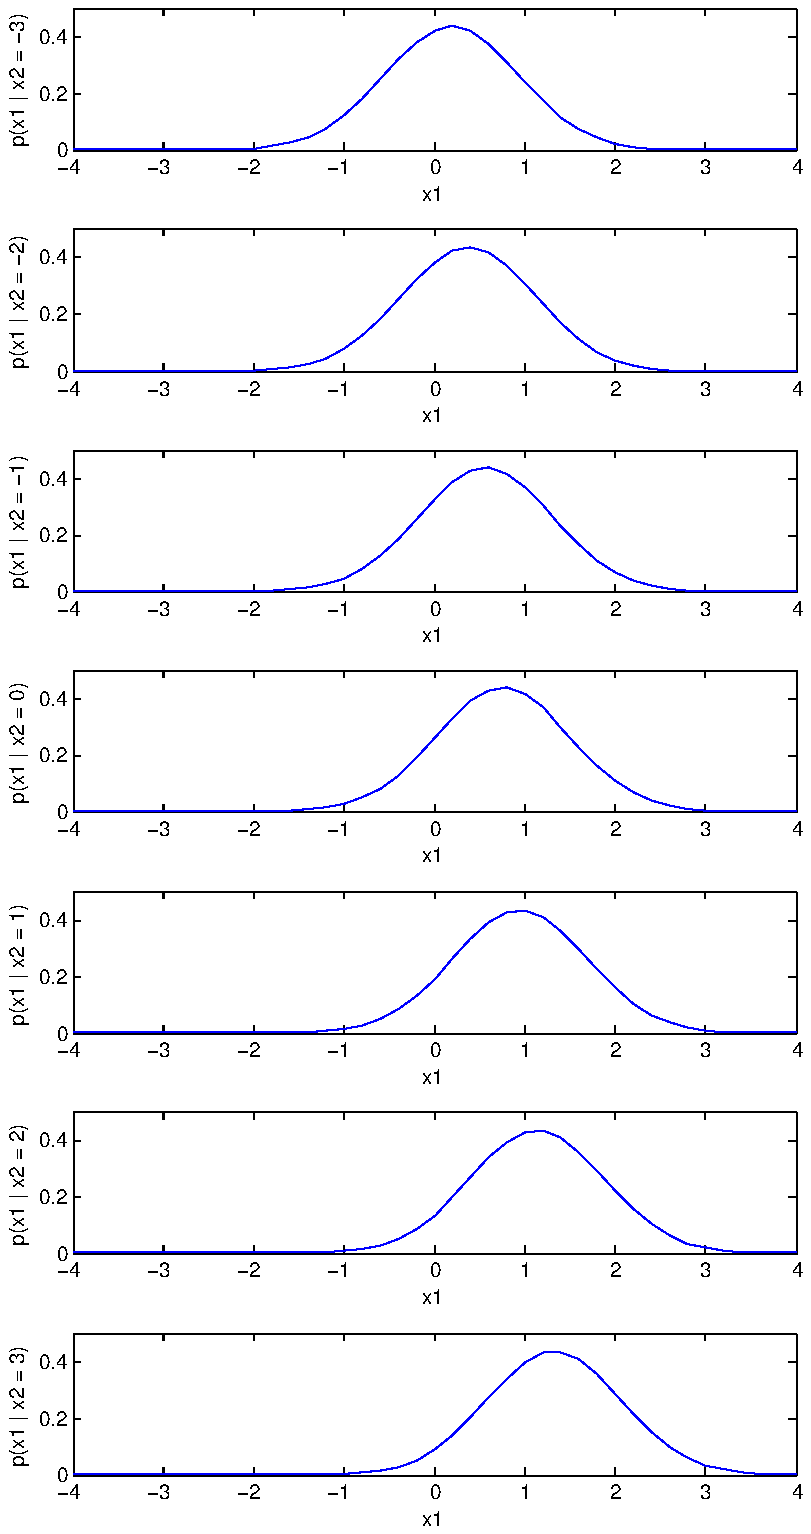
\includegraphics[width=0.8\textwidth]{ex1plot4}
  \end{center}
\end{figure}


In the first assignment, I have looked at a Gaussian distribution $\mathcal G_1 = \npdf(\V{X}; \mean, \cov)$ over two-dimensional vectors of real numbers.  The mean $\mean$ has been set to $0$, and the covariance $\cov$ to $\begin{bmatrix}1&0\\0&3\end{bmatrix}$.  The \hl{contour plot} of $\mathcal G_1$ has been plotted for input $\langle x_1, x_2 \rangle \in \V{X}$ where $-4 \leq x_1 \leq 4$ and $-4 \leq x_2 \leq 4$ in the \hl{upper part of \autoref{fig:plot1}}.  The lower part of \autoref{fig:plot1} presents the \hl{marginal distribution over }$\mhl{x_1}$.  This has been computed as $\mhl{\npdf(x_1; \mu_1, \Sigma_{1,1}) = \npdf(x_1; 0, 1)}$. 

  In \autoref{fig:plot2}, \hl{the marginal distribution} over $x_1$ for the follow values of $x_2$ are given, \hl{from top to bottom:} $\mhl{-3, -2, -1, 0, 1, 2, 3}$.  Not that these seven plots are identical to the subfigure in \autoref{fig:plot1}.  This is not really surprising, when looking at the computation:
  \begin{align*}
    p(x_1 | x_2 = v) 
    &= \npdf(x_1; \mean_1 - \Lambda_{1,1}^{-1} \Lambda_{1,2} (x_2 - \mu_2), \Lambda_{1,1}^{-1}) \\
    &= \npdf(x_1; 0 - 1  \times 0 \times v, 1) \\
    &= \npdf(x_1; 0, 1) \\
    &= p(x_1)
  \end{align*}
  with $\V{\Lambda} = \cov^{-1}$.

  Another distribution I have looked at, is $\mathcal G_2 = \npdf(\V{X}; \mean, \cov)$ with $\cov = \begin{bmatrix}1 & 0.7 \\ 0.7 & 1\end{bmatrix}$.  The \hl{surface plot is given in \autoref{fig:plot3}}.  Although the marginal distribution of $\mathcal G_1$ over $x_1$ and $\mathcal G_2$ are equal, their conditional distributions over $x_1$ given $x_2$ are not.  For $x_2 = v$, the conditional distribution is:
    \begin{align*}
      p(x_1 | x_2 = v)
      &= \npdf(x_1; \mean_1 - \Lambda_{1,1}^{-1} \Lambda_{1,2} (x_2 - \mu_2), \Lambda_{1,1}^{-1}) \\
      &= \npdf(x_1; 0 - 1.1952 \times -0.2789 \times x_2, 1.1952) \\
      &= \npdf(x_1; 0.3333 x_2, 1.1952)
    \end{align*}
\hl{The conditional distribution} over $x_1$ for $x_2 \in \left\{-3, -2, -1, 0, 1, 2, 3\right\}$ is presented in \hl{\autoref{fig:plot4}}.


\section{Gaussian Processes}

\end{document}
